\documentclass[twocolumn,10pt]{article}

%\usepackage{times}
\usepackage{fullpage}
\usepackage{eprint}
\usepackage{rotating}
\usepackage{eepic}
\usepackage{amsfonts}
\usepackage{algorithmic}
\usepackage{amsthm}

\theoremstyle{plain}
\newtheorem{theorem}{Theorem}

\title{Quantum Compiling with the Super-Kitaev Algorithm}
\date{February 11, 2011}
\author{Paul Pham}

\input{Qcircuit}

\begin{document}

%\newcommand{\ket}[1]{|#1 \rangle}
%\newcommand{\bra}[1]{\langle #1 |}
\newcommand{\braket}[2]{\langle #1|#2 \rangle}
\newcommand{\normtwo}{\frac{1}{\sqrt{2}}}
\newcommand{\norm}[1]{\parallel #1 \parallel}

\maketitle

\section{Abstract}

Quantum compilers will be needed to implement algorithms on an
80-qubit quantum computer being constructed in the next five years.
Like digital computers, quantum
computers need compilers to approximate high-level descriptions of
an algorithm using a low-level, universal, machine-dependent
instruction set. This work contributes
a numerical comparison of the
resources needed to run two separate quantum compiling algorithms, along
with the underlying open source code.
The first is the well-known Solovay-Kitaev theorem which showed that
efficient quantum compiling was possible in theory, but with some large
performance overheads in practice. The other is a
lesser-known result known as Super-Kitaev, which optimizes the compiled
circuit depth using parallelization at the expense of more ancilla qubits
and a larger overall circuit size. Finally, we discuss some implications for
future quantum architectures and also analog computers
(for when they come back into
fashion).


\section{Introduction}

Quantum computers can do some pretty amazing things in theory: they
can break the RSA cryptosystem using Shor's factoring algorithm,
ensure perfectly private communication,
do unstructured search, solve random walks, and
simulate quantum physical systems much more efficiently than classical
computers. But how
do we bridge the gap between algorithms that run on paper and those that
will soon run on actual machines being built in laboratories as we speak?
One important step in that direction is \emph{quantum compiling}, the
approximation of a high-level quantum algorithm description to a sequence
of low-level, universal quantum gates that depend on our hardware, the
"assembly language" of quantum computing.

When describing a quantum algorithm, we use a high-level formalism of
gates operating on qubits in the quantum circuit model.
We can treat gates operating on an $n$-qubit quantum computer as unitary
matrices of dimension $2^n \times 2^n$ with unit determinant.
However, in experimental settings,
we can only perform some gates efficiently, and these are local
two-qubit or single-qubit operations.
Moreover, most of our results for fault-tolerant
quantum computing in the presence of noise stipulates that we have a finite
number of universal gates we can perform with some limited precision.

Two quantum compiling algorithms are currently known. The first algorithm,
by Solovay and Kitaev \cite{Dawson2005},
is one of the central results of quantum computing which states that we
can approximate quantum gates efficiently without losing any performance
gains over classical computers.
The second result, which is more recent but much less well-known, improves
Solovay-Kitaev by making a time-space tradeoff and using parallelism
\cite{ksv02}.
Therefore, we call it Super-Kitaev (a name originated by Aram Harrow).

This work contributes the calculation of physical resources needed
to run these two quantum compiling algorithms, open source code to duplicate
these results available at \texttt{http://quantum-compiler.org},
and much needed publicity for Super-Kitaev.

The rest of this report is organized as follows.
First things first, Section \ref{sec:prelims} defines terms and parameters
so that we can discuss quantum compilers with some precision as well as
giving asymptotic bounds for specific algorithms.
Then Section
\ref{sec:related} gives a brief history of quantum compiling.
The next two sections describe the two compiling algorithms and how
to measure their relative performance.
Section \ref{sec:sk-algo} reviews the original Solovay-Kitaev result and
Section \ref{sec:main-algo} describes Super-Kitaev along with its
most resource-intensive modules. Section \ref{sec:methods} describe
our methods for the performance comparisons, which are given in Section
\ref{sec:results}. Finally, we make some comments about these results
and suggest future directions for extending this work. Ready? Let's go.

\section{Definitions}

\subsection{Approximation vs. Simulation}

I'll use the terms "approximation" and "simulation" interchangeably, as in
a quantum compiler will take an input circuit and produce as output a new
circuit which approximates or simulates the original circuit to some degree
of precision.

\subsection{Standard Set}

We use the following standard set $\mathcal{Q}$ from \cite{ksv02}

\begin{equation}
\mathcal{Q} = \{ H, K, K^{-1}, \Lambda(\sigma^x), \Lambda^2(\sigma^x) \}
\end{equation}

where these gates are defined as follows:

\begin{equation*}
H = \normtwo \left(
  \begin{array}{cc}
    1 & 1 \\
    1 & -1 \\
  \end{array} \right)
\end{equation*}

\begin{equation*}
K = \left(
  \begin{array}{cc}
    1 & 0 \\
    0 & i \\
  \end{array} \right)
\end{equation*}

Even though realistic implementations of a quantum computer may have a different
set of hardware instructions, Kitaev's analysis assumes that the standard set
can always be efficiently compiled down further into this hardware set.

Note that this may not be valid. For example, in order for ion traps to perform
even a Hadamard gate to any precision requires a combination of $\sigma^x$ and
$\sigma^z$ gates. However, we won't let this bother us for now.

\subsection{Parameters}

For these notes, we restrict ourselves to $d=2^n$ for an $n$-qubit system (qudits)
and consider the problem of compiling an entire circuit $C$ of $L$ gates with depth
$d$ to a new, compiled circuit $C'$ of size $L'$ and depth $d'$ which approximates
$C$ within some error. There is some overhead in the compiled circuit, so in
general $C'$ is larger (that is, $L' > L$ and $d' > d$). It's also known that
in order to approximate a circuit with $L$ gates to a total precision of $\epsilon$
requires each gate to be approximated to a precision of $L/\epsilon$, which requires
the following number of gates. We'll find this $l$ parameter useful in describing the compiler overheads of
both the Solovay-Kitaev and Super-Kitaev methods.

Why do we care about depth? This gives us a heuristic for how ``parallelized'' our
circuit is. If we flatten our circuit into layers $\{l_i\}$, where each layer $l_i$
is dependent only on inputs from the previous layer $l_{i-1}$ and produces
only outputs to the next layer $l_{i+1}$, then all the gates within the layer
$l_i$ can be performed in parallel. All other things being equal, a circuit with low depth will complete
faster than one with high depth, although in practice we can only execute
fixed-width circuits.

Also, when running the compiler, there are several time resources to consider.
The first is classical preprocessing time, denoted $T_{pre}$, which is a way of optimizing
the generated quantum circuit by spending more classical resources upfront.
The second is classical postprocessing time, denoted $T_{post}$, which likewise
is meant to reduce the size of the quantum circuit but depends on quantum
measurements and may be fed back into future quantum operations later.

A summary of these parameters are provided below:

\begin{tabular}{|c|c|}
\hline
$d$ & dimension of quantum gates (matrix representation)\\
$\epsilon$ & the desired accuracy of the compiled circuit\\
$L$ & size of input circuit to be compiled, in gates from $\mathcal{Q}$\\
$d$ & depth of input circuit to be compiled\\
$L'$ & size of compiled output circuit, in gates from $\mathcal{Q}$\\
$d'$ & depth of compiled circuit to be compiled\\
$n$ & $=O(\log{L/\epsilon})$, shorthand parameter for asymptotic analysis\\
$T$ & classical running time of the compiling algorithm\\
$T_{pre}$ & classical preprocessing time, before the compiler is run\\
$T_{post}$ & classical postprocessing time, after the compiler is run or during\\
\hline
\end{tabular}

\subsection{Universal Instruction Sets and Compiled Sequences}
More formally, suppose we have a universal instruction set $\mathcal{G}$ which
contains some finite number of gates $g \in SU(d)$ and also their inverses $g^\dagger$.
$\mathcal{G}$ is universal for $SU(d)$ in that it generates a dense subgroup.
In other words, given an arbitrary quantum gate $U \in SU(d)$ and a desired
accuracy $\epsilon$ we can find a product $S=g_1 \cdots g_m$ from $\mathcal{G}$
which approximates $U$ to within $\epsilon$ using some distance function.

We can either use the matrix operator norm to define the distance function
such as:

\begin{equation}
d(U,S) \equiv \norm{U - S} \equiv \sup_{\norm{\ket{\psi}}=1} \norm{(U-S)\ket{\psi}} < \epsilon
\end{equation}

There is also a trace measure introduced by Austin Fowler which disregards
the global phase factor, so that we don't waste time trying to approximate
the unmeasurable phase of our target gate.

\begin{equation}
d(U,S) = \sqrt{\frac{d - \norm{\mathrm{tr}(U^\dagger S)}}{d}}
\end{equation}

\subsection{Some Special Operator Notation}

As I've become fond of the notation in \cite{ksv02}, I borrow the
following notation for two "meta-operators" which takes some unitary $U$ as
a parameter. The first describes a controlled-$U$ operation where the control
is some single qubit.

\begin{displaymath}
\Lambda(U) = \ket{0}\bra{0} \otimes I + \ket{1}\bra{1} \otimes U
\end{displaymath}

The second describes a registered-$U$ operation, which
can be thought of as controlled on some multi-qubit register $\ket{p}$
encoding an $m$-qubit number $p$ to apply $U$ a certain number of times to a
target
register.

\begin{displaymath}
\Upsilon_m(U) : \ket{p} \otimes \ket{\psi} \rightarrow \ket{p}
\otimes U^p\ket{\psi}
\end{displaymath}


%\section{Performance}

Just to get this out of the way, in case you are wondering whether to be
excited or not about Super-Kitaev.

\begin{tabular}{|c|c|c|}
\hline
   & Solovay-Kitaev & Super-Kitaev\\
$L'$ & $O(Ln^{3+\nu})$ & $O(Ln + n^2 \log n)$\\
$d'$ & $O(dn^{3+\nu})$ & $O(d \log{n} + (\log{n})^2))$\\ 
\hline
\end{tabular}

where $\nu$ is a small positive constant.
The remaining parameters are yet to be determined.



\section{Related Work}
\label{sec:related}

In 1995, Seth Lloyd found that almost any two distinct single-qubit rotations are
universal for approximating an arbitrary single-qubit rotation, but that this
approximation could be exponentially long in both time and length $T,L = (O(1/\epsilon))$ \cite{Lloyd1995}.

The theorem which is now called Solovay-Kitaev was discovered by Solovay in
1995 in an unpublished manuscript and independently later discovered by
Kitaev in 1997 \cite{nc00} which showed that $T,L = O(\log^c{1/\epsilon})$ for
$c$ between 3 and 4.

In 2001, Aram Harrow completed his undergrad thesis arguing that it would be difficult
to beat $c < 2$ for the above bounds using a successive approximation
method\cite{harrow01}.

In 2002, Kitaev, Shen, and Vyalyi published their book which contains an
application of parallelized phase estimation towards simulating a quantum
circuit (what we are calling Super-Kitaev) \cite{ksv02}.
That is, an alternative quantum compiler to Solovay-Kitaev which has
asymptotically better circuit depth and $T=O(1)$
but using ancillary qubits and increased
circuit size.

In 2003, Harrow, Recht, and Chuang demonstrated that a certain universal
set could be used to saturate the lower bound $L=O(\log{1/\epsilon})$
but it remains an open problem whether any efficient algorithm exists
which can do this in tractable $T$ \cite{hrc02}.

In 2005, Dawson and Nielsen published their pedagogical review
paper of Solovay-Kitaev \cite{Dawson2005}.

In 2010, Burrello, Mussardo, and Wan discovered a quantum compiler for
topological quantum computing which saturates the lower bound ($c=1$) for
non-Abelian anyons \cite{Burrello2010}.

\section{Review of Solovay-Kitaev}

Here I'll remind you of the basic pseudo-code for normal Solovay-Kitaev.
Our development is taken from the excellent review paper \cite{Dawson2005}.

\begin{algorithmic}[1]
\STATE \textsc{function} $\tilde{U}_n \leftarrow$ SOLOVAY-KITAEV$(U,n)$
\IF{$n == 0$}
\STATE $\tilde{U}_n \leftarrow $ BASIC-APPROX$(U)$
\ELSE
\STATE $\tilde{U}_{n-1} \leftarrow$ SOLOVAY-KITAEV$(U, n-1)$
\STATE $A,B \leftarrow $ FACTOR$(U\tilde{U}^\dagger_{n-1})$
\STATE $\tilde{A}_{n-1} \leftarrow $ SOLOVAY-KITAEV$(A, n-1)$
\STATE $\tilde{B}_{n-1} \leftarrow $ SOLOVAY-KITAEV$(B, n-1)$
\STATE $\tilde{U}_n \leftarrow \tilde{A}_{n-1}\tilde{B}_{n-1}\tilde{A}^\dagger_{n-1}\tilde{B}^\dagger_{n-1}\tilde{U}_{n-1}$
\ENDIF
return $\tilde{U}_n$
\end{algorithmic}

This algorithm works by way of recursive, successive approximation.

The BASIC-APPROX function above does a lookup (via some kd-tree search
maneuvers through higher-dimensional vector spaces) using the results of
precompiled sequences from the instruction set $\mathcal{G}$. This can be
done offline and reused across multiple runs of the compiler, assuming
$\mathcal{G}$ for your quantum computer doesn't change.

The FACTOR function performs a balanced group commutator decomposition,
$U = ABA^\dagger B^\dagger$, and then recursively approximates the $A$ and $B$
operators using Solovay-Kitaev. Intuitively, when they are multiplied
together again, along with their inverses, their errors (which go like
$\epsilon$) are symmetric and cancel out in such a way that the resulting
product $U$ has errors which go like $\epsilon^2$. In this manner, we can
eventually sharpen our desired error down to any value.

And that's all I'm going to say about that.


%\section{The Super-Kitaev Algorithm}

Our development of the Super-Kitaev algorithm follows closely the one in the
book by Kitaev, Shen, and Vyalvi \cite{ksv02}, although of course, it is
simply called Theorem 13.5. Likewise, we will cite the theorem / lemma numbers
from the book, which contains a self-contained description of all the parts
needed for Super-Kitaev.

The basic steps of this method are the following:

\begin{enumerate}
\item Precompiling to get $L'$ gates in $\mathcal{Q} \cup \Lambda(e^{i\phi})$.
Here we see that there is an
efficient decomposition of several important gates into the standard set and
controlled-phase-shifts.
\item Implementing a controlled-phase-shift. This ends up being the hardest
part of simulating a quantum circuit, and requires each of the remaining steps.
\item Use phase estimation of an addition operator to magic states in order to
enact the desired phase shift. This requires both efficient creation of
{\em magic states} and an efficient {\em quantum adder} circuit.
\item Create one magic state, and then make $L'$ copies of it. Use one copy
to simulate each $\Lambda(e^{i\phi})$ gate.
\end{enumerate}


\section{The Main Algorithm}
\label{sec:main-algo}

The Super-Kitaev algorithm takes a radically different approach than
Solovay-Kitaev by identifying that most gates can be easily reduced to
$\mathcal{G}$ in constant time with the exception of the ``targetless''
controlled phase operator, which will take some sweat to approximate.

\begin{displaymath}
\Lambda(e^{i\phi}) = 
 \left(
  \begin{array}{cc}
    1 & 0 \\
    0 & e^{i\phi} \\
  \end{array} \right)
\end{displaymath}

Thankfully \cite{ksv02} is a self-contained reference
for enacting $\Lambda(e^{i\phi})$ with several modules which are useful in
their own right:
parallelized phase estimation procedure, parallel iteration of finite
automata, and a logarithmic depth quantum arithmetic operations such
as addition (and subtraction) described in \ref{subsec:add},
multiplication described in \ref{subsec:mult}, and division described
in \ref{subsec:div}.

It is now useful to discuss certain states with magical properties.
Their superposition is easy to form, they are the eigenstates of the
afore-mentioned
addition operator. Used with phase estimation, this would allow us to enact
a random phase shift simply by adding numbers, which is better than not
being able to shift phases at all (or only being able to do it with a
complicated operator). Moreover, it turns out we can copy these states
also using simple addition. These ideas make Super-Kitaev a beautiful result
regardless of the outcome of our later numerical comparisons.

\subsection{Magic States}
\label{subsec:magic-state}

Suppose you had some magic state $\ket{\psi}$, given to you from some
all-powerful being, parameterized by the
integers $n$ and $k$ such that

\begin{equation*}
\ket{\psi_{n,k}} = \frac{1}{\sqrt{2^n}} \sum_{j=0}^{2^n-1}
e^{-2\pi i j k / 2^n} \ket{j}
\end{equation*}

where $0 < k < 2^n$, $k$ is odd.

Note that the magic states $\ket{\psi}$ look suspiciously like a
QFT state of the computational basis.
However that doesn't help us here, because QFT in general requires
$O(n^2)$-depth and we need a logarithmic-depth compiler.
This is intuitively why these states are hard to create.
If we were able to construct them easily, we would also have a quicker way
of implementing QFT.

However, what we can do is create a superposition over all odd $k=(2s-1)$
by starting in the state $\ket{0}^{\otimes n}$,
applying a Hadamard to the most significant qubit to get an equal mix of $\ket{0}$
and $\ket{1}$, then put a negative sign on the $\ket{1}$ component by applying
$\sigma^z$ to the same qubit.

\begin{equation*}
\ket{\eta} = \normtwo \ket{0} - \normtwo \ket{2^{n-1}} =
\frac{1}{\sqrt{2^{n-1}}} \sum_{s=1}^{2^{n-1}} \ket{\psi_{n,2s-1}}
\end{equation*}

More obviously relevant to our overall goal of approximating
$\Lambda(e^{i\phi})$, we can enact a phase
shift simply by doing addition, which is a result of these states
being eigenvectors of the modular addition operator defined
%by $A : \ket{j} \rightarrow \ket{(j+1) mod 2^n}$
 
\begin{equation*}
A\ket{\psi_{n,k}} = e^{2\pi i \phi_k} \ket{\psi_{n,k}}
\end{equation*}

\begin{equation*}
A\ket{j} \rightarrow \ket{j+1 \mod 2^n}
\end{equation*}

where finding the eigenvalue $e^{2\pi i \phi_k}$ corresponds to finding
the phase $\phi_k = k / 2^n$.

Repeated application of $A$ (say $p$ times) would result in a phase
added to the eigenstate equal to a multiple of $e^{2\pi i p / 2^n}$

\begin{equation}
A^p\ket{\psi_{n,k}} = e^{2\pi i \phi_k / 2^n} \ket{\psi_{n,k}}
\end{equation}

This explains why we don't find even $k$ interesting,
since then we would not get a
cyclic distribution of $2^n$ different phases,
since only odd $k$
are coprime with $2^n$. The exception is $k=0$, since this is the
equal superposition of computational basis states, which we can also
efficiently create. This will be a useful starting point later on to
create magic states
for odd $k$.

\begin{displaymath}
\ket{\psi_{n,0}} = H^{\otimes n}\ket{0^n}
\end{displaymath}

Suppose we have a certain state $\psi_{n,k}$ but we want to get enact
a phase shift $e^{2\pi i l / 2^n}$. We can do this by solving $p=p(s,l)$
in this equation:

\begin{equation}
\label{eqn:psl}
(2s-1)p \equiv l (\mod 2^n)
\end{equation}

Stipulating $k$ to be odd guarantees that there is a unique solution $p$.

We then applying $A^p$ as follows:

\begin{equation}
\label{eqn:upsilon}
\Upsilon_n(A) \ket{p, \psi_{n,k}} \rightarrow
e^{2\pi i l/2^n} \ket{p, \psi_{n,k}}
\end{equation}

But $p$ is in general hard to solve for, unless $k=1$, in which case
$p = l$. Therefore, we will later see that $\ket{\psi_{n,1}}$ is a desirable
state to have.

Finally, to copy the state $\ket{\psi_{n,k}}$ it suffices to apply the following
operator which only uses subtraction (addition with one addend and the
outcome negated in two's complement representation).

\begin{equation*}
\ket{\psi_{n,k}}^{\otimes m} = W^{-1}\left( \ket{\psi_{n,0}}^\otimes(m-1) \otimes \ket{\psi_{n,k}} \right)
\end{equation*}

where $W$ is defined by

\begin{multline}
W : \ket{x_1,\ldots,x_{m-1},x_m} \rightarrow \\
 \ket{x_1,\ldots,x_{m-1},x_1+\ldots+x_m}
\end{multline}

Armed with these properties, we're now ready to enact arbitrary phase shifts.

%For the steps below, we note that we can avoid solving the equation $kp \equiv l (mod 2^n)$
%if we set $k=1$. This is equivalent to realizing $\Upsilon_n(e^{2\pi i / 2^n})$
%by applying $\Upsilon(A)$ from Section \ref{subsec:phase-shift} to the state
%$\ket{\psi_{n,1}}$. So we need to create one copy of this magic state to
%simulate each of $m$ $\Lambda(e^{i\phi})$ gates, $m \le L'$.


\subsection{Super-Kitaev Steps}

Given a circuit $C$ to compile,

\begin{enumerate}
\item Precompile $C$ into gates from $\mathcal{G} \cup \{\Lambda(e^{2\pi i l / 2^n})\}$
using the results from Section \ref{subsec:precompile} in $O(1)$ time, depth,
and size.
Now we are done with the single-qubit gates and CNOT, and we have computed
the values $\{l_1, \ldots , l_m\}$ that allow us to approximate our
desired $m$
$\Lambda(e^{i\phi})$ gates as $\phi \approx l/2^n$ to within precision
$2^{-n}$.
\item Create the state magic state $\ket{\psi_{n,0}}$ with $n$ Hadamards.
\item Turn it into $\ket{\psi_{n,1}} = \Upsilon(e^{-2\pi i / 2^n}) \ket{\psi_{n,0}}$
using the registered phase shift procedure in Section \ref{subsec:phase-shift}
This is done with a circuit of size $O(n^2\log n)$ and $O((\log n)^2)$ depth.
\item Make $m$ copies of the state $\ket{\psi_{n,1}}$ out of one copy by 
applying the addition operation $A$.
\item Simulate each $\Lambda(e^{2\pi i l / 2^n})$
using one copy each of $\ket{\psi_{n,1}}$, to which we can add our
values $l$ using $\Upsilon(A)$.
This takes size $O(mn)$ and depth $O(\log n)$, since we can enact
all these phase shifts in parallel.
\end{enumerate}

Now for the resource calculations of these individual steps and their
substeps.

\subsection{Precompiling to the Standard Set}
\label{subsec:precompile}

This is the completely classical preprocessing step for Super-Kitaev which
assumes we can express any $n$-qubit gate as a tensor product of
single- and two-qubit gates.
From there, how do we get down to our universal set?

%\begin{theorem}[Lemma 8.2]
%\label{lemma82}
%Any arbitrary unitary operator $U$ of dimension $d \times d$ can be represented
%as a product of $d(d-2)/2$ matrices of the form:
%
%\begin{equation*}
%\left( \begin{array}{cccccccc}
%     1 & 0      & \cdots & \cdots & \cdots & \cdots & \cdots & \cdots\\
%     0 & 1      & \cdots & \cdots & \cdots & \cdots & \cdots & \cdots\\
%\vdots & \cdots & \ddots & \cdots & \cdots & \cdots & \cdots & \cdots\\
%\vdots & \cdots & \cdots &      a &      b & \cdots & \cdots & \cdots\\
%\vdots & \cdots & \cdots &      c &      d & \cdots & \cdots & \cdots\\
%\vdots & \cdots & \cdots & \cdots & \cdots & \vdots & \cdots & \cdots\\
%\vdots & \cdots & \cdots & \cdots & \cdots & \cdots & 1 & 0\\
%\vdots & \cdots & \cdots & \cdots & \cdots & \cdots & 0 & 1\\
%\end{array}
%\right)
%\end{equation*}
%
%where $\left( \begin{array}{cc}
%a & b\\
%c & d\\
%\end{array} \right) \in SU(2)$
%\end{theorem}
%
%\begin{proof}
%The running time of this algorithm is $O(M^3) \cdot \mathrm{poly}(\log(1/\delta)$.
%\end{proof}

We use the Euler angle decomposition into $X$ and $Z$ rotations,
we can express any
unitary $U$ as follows, with real angles $\phi$, $\gamma$, $\beta$, $\alpha$:

\begin{equation*}
U = e^{i\phi}e^{i(\gamma/2)\sigma^z}e^{i(\beta/2)\sigma^x}e^{i(\alpha/2)\sigma^z}
\end{equation*}
This involves solving four equations in four variables and can be done in
constant time.

Now how do we implement each of the elements of the Euler angle decomposition from
the $\mathcal{Q}$? Using these identities:

\begin{equation*}
e^{i\phi} = \Lambda(e^{i\phi})\sigma^x\Lambda(e^{i\phi})\sigma^x
\end{equation*}
\begin{equation*}
\sigma^x = H\Lambda(e^{i\pi})H
\end{equation*}
\begin{equation*}
e^{i\phi\sigma^z} = \Lambda(e^{-i\phi}\sigma^x\Lambda(e^{i\phi})\sigma^x
\end{equation*}
\begin{equation*}
e^{i\phi\sigma^x} = H e^{i\phi\sigma^z} H
\end{equation*}

In addition,
any controlled operator $\Lambda(U)$ where $U \in SU(2)$ can be simulated
using
$\mathcal{Q} \cup \{ \Lambda(e^{i\phi})$.

We can represent the controlled operator as $\Lambda(U) = \Lambda(e^{i\phi})\Lambda(V)$.
$\Lambda(e^{i\phi})$ is already in our set, so it remains to implement
$\Lambda(V)$, where $V \in SU(2)$. Geometrically, we can decompose any
three-dimensional rotation into two $180^{\circ}$ rotations about appropriate
axes. Using the homomorphism between $SO(3)$ and $SU(2)$ and the fact that
$\sigma^x$ corresponds to a $180^{\circ}$ rotation about the $x$-axis.

\begin{equation*}
V = A\sigma^x A^{-1} B\sigma^x B^{-1}
\end{equation*}


\subsection{Controlled-Phase Shift}
\label{subsec:phase-shift}

Now we are down to the standard set $\mathcal{Q}$, plus that pesky
controlled-phase-shift gate $\Lambda{e^{i\phi}}$. This is in general a hard
gate to implement, and one of the reasons why we need a quantum compiler in
the first place!

We could just use normal Solovay-Kitaev and find some sequence of $X$ and
$Z$ gates which implement $\Lambda{e^{i\phi}}$, but that wouldn't be any
fun and we would have no reason to bring in all this extra machinery to
do Super-Kitaev.

Note that in general we can't exactly implement $\Lambda{e^{i\phi}}$ but we
can approximate it as $\Lambda{e^{2\pi i l / 2^n}}$, where $l$ is an integer.
In general this is a special case of the following operator
defined by Kitaev in the following lemma.

\begin{theorem}[Lemma 13.4]
The operator 
$\Upsilon_n(e^{2\pi i / 2^n}) : \ket{l} \rightarrow e^{2\pi i l / 2^n} \ket{l}$
for $0 \le l < 2^n$ can be realized with precision $\delta = 2^{-n}$ by an
$O(n^2 \log n)$-size $O((\log n)^2)$-depth circuit over the standard basis
using ancillas.
\end{theorem}

\begin{proof}
To get started, we will need to introduce a magic state $\ket{\psi}$ with the
integer parameters $n$ and $k$ such that

\begin{equation}
\ket{\psi_{n,k}} = \frac{1}{\sqrt{2^n}-1} \sum_{j=0}^{2^n-1} e^{2\pi i j k / 2^n} \ket{j}
\end{equation}

where $0 \le k < 2^n$, $k$ is odd.

What is interesting to note about this state is that we can enact a phase
shift simply by doing addition. In fact, addition is so useful in Super-Kitaev
that we will later discuss a parallelized adder circuit which, however,
is generic enough to be useful in other quantum algorithms.

%What we need instead is to make use of the index-dependent
%phases of each state, and addition to move to the right phase that we want,
%and easy creation of a superposition of these magic states.

Note that this magic state is an eigenstate of the addition operator defined
by $A : \ket{j} \rightarrow \ket{(j+1) mod 2^n}$
 
\begin{equation}
A\ket{\psi_{n,k}} = e^{2\pi i \phi_k / 2^n} \ket{\psi_{n,k}}
\end{equation}

where finding the eigenvalue $e^{2\pi i \phi_k}$ corresponds to finding
the phase $\phi_k = k / 2^n$

Repeated application of $A$ (say $p$ times) would result in a phase
added to the eigenstate equal to a multiple of $e^{2\pi i p / 2^n}$

\begin{equation}
A^p\ket{\psi_{n,k}} = e^{2\pi i \phi k / 2^n} \ket{\psi_{n,k}}
\end{equation}

To realize our desired operator $\Upsilon_n{e^{2\pi i / 2^n}}$ it suffices
to use the value of $l$ to compute $p$ and then apply the operator:

\begin{equation}
\Upsilon_n(X) : \ket{p,j} \rightarrow \ket{p, (j+p) \mod 2^n}
\end{equation}

for $p,j \in {0,\ldots,2^n-1}$. That is, two $n$-qubit registers contain
the values $p$ and $j$.

Ideally, we would just create $\ket{\psi_{n,k}}$ for some particular $k$
($k=1$ would be ideal). Then we would know exactly which $\ket{\psi_{n,k}}$
we had, and how many times $p$ to apply the $A$ operator
to enact the desired phase shift, where $p$ is the solution to the
following equation:

\begin{equation}
\label{eqn:kp}
kp \equiv l (\mod 2^n)
\end{equation}

Note that we stipulate $k$ to be odd so that there is a unique solution $p$.

Recall now that the magic states $\ket{\psi}$ look suspiciously like a
Quantum Fourier Transform state of the computational basis.
However that doesn't help us here, because QFT is way too complicated to use as
our basic compiler. This is intuitively why these states are hard to create.
If we were able to construct them easily, we would also have a quicker way
of implementing QFT.

However, what we can do is create a superposition over all odd $k$ in the
following way:

\begin{equation}
\ket{\eta} = \normtwo \ket{0} - \normtwo \ket{2^{n-1}} =
\frac{1}{\sqrt{2^{n-1}}} \sum_{s=1}^{2^{n-1}} \ket{\psi_{n,2s-1}}
\end{equation}

Now then here are the required steps.

\begin{enumerate}
\item Create the state $\ket{\eta}$ by starting in the state $\ket{0}^{\otimes n}$,
applying a Hadamard to the most significant qubit to get an equal mix of $\ket{0}$
and $\ket{1}$, then put a negative sign on the $\ket{1}$ component by applying
$\sigma^z$ to the same qubit.
\item Measure $k$ by determining the phase $\phi_k = k/2^n$ with precision
$\delta = 2^{-n}$ by using phase estimation. One of the $n$-qubit registers
now contains $\ket{\psi_{n,k}}$ for some fixed $k$.
This is done by a circuit of size $O(n^2)$ and depth $O(\log n)$.
\item Solve for $p$ as a function of $k$ and $l$ satisfying Equation \ref{eqn:kp}
\item Apply $X^p$ to the $n$-qubit register containing $\ket{\psi}$, which
enacts the desired phase shift.
\item Reverse the first three steps to uncompute $p$
\end{enumerate}

Note that we skimmed over the solution to Equation \ref{eqn:kp} even though this
is the most resource-intensive part of the algorithm. Rest assured, it reduces
to division (or computing the inverse of $2s-1 \mod 2^n$) which Kitaev
provides an efficient solution to as Problem 2.14a in his book.

\end{proof}


\subsection{Parallelized Phase Estimation}
\label{subsec:ppe}

One of the key components of the registered phase shifting procedure
described in the previous section is the ability to ``pick'' a random
eigenstate $\ket{\psi_k}$ of a unitary operator $U$ and
measure its corresponding eigenvalue (phase) $\phi_k$
with some degree of precision $\delta = 2^{-n}$ and
error probability $\epsilon = 2^{-l}$. As $n$ increases, the phases
generally become closer together, which is why we need exponential precision
to distinguish between them.
Of course, this exactly describes the phase
estimation procedure, a key technique in many quantum algorithms developed
by Kitaev in his derivation of Shor's factoring result \cite{kitaev}.

\begin{displaymath}
U\ket{\psi_k} = e^{2\pi i \phi_k} \ket{\psi_k}
\end{displaymath}

Phase estimation holds some superposition of eigenstates
$\sum_{i} \alpha_i \ket{\psi_i}$
in an $n$-qubit target register, to which it applies repeated measuring
operators $\Lambda(U^{2^k})$
controlled on some $t$-qubit register, which holds an
approximation $\tilde{phi}$ to the real phase $\phi$.
The unitary $U$ is applied in successive powers of two to get
power-of-two multiples of the phase for increased precision.
The error probability of approximating the phase to within a given
precision is given by the following:

\begin{displaymath}
\Pr\left[ | \phi - \tilde{phi} | \ge \delta \right] \le \epsilon
\end{displaymath}

The parameter $t = t(\delta, \epsilon)$ encodes the dependence of the number
of $\Lambda(U)$ measuring operators as a function of our desired
$\delta$ and $\epsilon$.
It varies according to the exact phase estimation procedure
used.

The popular version of phase estimation presented in \cite[nc00],
requires $t$ repeated controlled applications of some unitary
$U$ (and its successive powers as $U^{2^k}$, $0<k<2^t$)
to a target state which holds some superposition of its eigenvectors,
controlled by $t$ bits which will hold the approximation to a corresponding
eigenvalue (phase).
This version requires applying an inverse quantum Fourier
transform (QFT), which is already high-depth and way more inefficient than our
desired quantum compiler.

To achieve our desired low-depth, we can ``parallelize'' the application of
$\Lambda(U)$ by interpreting the
$t = (n+2)s$ control bits as an $n$-bit number $q$ and
apply $\Lambda(A^q)$ only once.
In the Super-Kitaev procedure, $A$ is the addition operator on an $n$ qubit
target register containing $\psi_{n,k}$, so we can
only effectively add the lowest $n$ bits of $q$.
Furthermore, the eigenvalues of $A$ are rational with a fixed
denominator, $\phi_k = k / 2^n$.
To avoid the inverse QFT,
we can do a classical postprocessing step, which we'll mostly skip over
for fairly good reasons, and then we'll do a detailed resource count of
parallelized phase estimation.

\subsection{Classical Postprocessing}

It is now the point to mention that Kitaev's phase estimation procedure
contains a post processing step which is completely classical in
character, in that they involve a measurement. If this measurement is
projective and the outcomes are completely classical, the remaining steps
can be done on our classical computer (recall our quantum coprocessor model),
and the results fed back into our quantum subroutine, registered
phase shifting. Therefore, as long as we can perform these classical
algorithms in polynomial time (which we can), we don't really care
about the equivalent circuit size and depth.

The steps of classical postprocessing, which will determine some of the
parameters in the earlier, quantum part of phase estimation are as follows.

\begin{enumerate}

\item
Estimate the phase and its power-of-two multiples
$2^j \phi_k$ to
some constant, modest precision $\delta''$, where
$0 \le j < (n+2)$. For each $j$, we
apply a series of $s$ measuring operators targeting the state $\ket{\nu}$
controlled on $s$ qubits in the state $(\ket{0}+\ket{1})/\sqrt{2}$,
essentially encoding the $2^j \phi_k$ as a bias in a coin, and flipping the
coin $s$ times in a Bernoulli trial, counting the number of $1$ outcomes,
and using that fraction to approximate the real $2^j \phi_k$.
\item
Sharpen our estimate to exponential precision $1/2^(n+2)$ using the
$(n+2)$ estimates, each for different bits in the binary expansion of
$phi_k$. Multiplication by successive powers-of-two shift these bits
up to a fixed position behind the zero in a binary fraction representation,
where we can use a finite-automata and a constant number of
bits to refine our $O(n)$-length running approximation.
\end{enumerate}

Three things are worth mentioning about the interrelation of the parameters
between these two steps. Since our phases all have a denominator of $2^n$,
there is no need to run the continued fractions algorithm on multiple
convergents, as is the case with period-finding in Shor's factoring algorithm.
Furthermore, the phases are $1/2^n$ apart, therefore it suffices to approximate
the phases to within $1/2^{n+2}$ in order to break ties, which is where
our range for $j$ comes from above.

The number of trials $s$ comes from the Chernoff bound:

\begin{displaymath}
\Pr \left[ | s^{-1}\sum_{r=1}^s v_r - p_* | \ge \delta'' \right]
\le 2e^{-2\delta'^2 s}
\end{displaymath}

Setting this equal to the desired error probabiliy $\epsilon$ we get

\begin{displaymath}
s = \frac{1}{2\delta''^2}\ln \frac{1}{\epsilon}
\end{displaymath}

We are actually estimating the values $\cos(2\pi \cdot 2^j \phi_k)$ and
$\sin(2\pi \cdot 2^j \phi_k)$, so if we wish to know $2^j \phi_k$ with
precision $\delta''$, we actually need to determine the $\cos(\cdot)$ and
$\sin(\cdot)$ values with a different precision $\delta'$, lower-bounding
it with the steepest part of the cosine and sine curves.

\begin{displaymath}
\delta' = 1 + cos(\pi - \delta'')
\end{displaymath}

The factor $\frac{1}{2\delta''^2}$ depends on the constant precision with
which we determine our $2^j \phi_k$ values. Since classical time is
cheap and quantum gates are expensive, it makes sense to minimize the number
of trials $s$. The following table shows the corresponding values of $1/(2\delta''^2)$
and $\delta'$ as a function of various choices for $\delta'$.

\begin{center}
\begin{table}
\begin{tabular}{|c|c|c|}
\hline
$\delta''$ & $\delta'$   & $1/(2\delta''2)$\\
\hline
$1/16$     & $0.0019525$ & $131,160$\\
$1/8$      & $0.0078023$ & $  8,213$\\
$1/4$      & $0.0310880$ & $    517$\\
\hline
\end{tabular}
\end{table}
\end{center}

By making our $\delta'$
exponentially worse (doubling it) we are only increasing the range of
$j$ a linear amount (by one). In general, for $\delta'=1/2^l$, we get
a final estimate for $\phi = 2^{m-3}$

However, projective measurements are irreversible, and we may wish to
uncompute the phase estimation procedure to restore our ancilla to
their initialized state and reuse them later on. In that case, the
postprocessing can actually be done on a quantum computer using
reversible gates and without projective measurements. That's why
the authors of \cite{ksv02} go to some care to show that all the classical
postprocessing steps can be done in polynomial-size and logarithmic-depth
circuit.
However, to simplify our analysis, we assume the case
in the previous paragraph, and accept the
loss of $n$ ancilla qubits, After all, we only run phase estimation once
to get our initial $\ket{\psi_{n,1}}$ state.

\subsection{Steps in the Parallelized Phase Estimation Algorithm}

The main steps in parallelized phase estimation as applied to Super-Kitaev
are:

\begin{enumerate}

\item Begin with a $t$-qubit ancilla register initialized to $\ket{0}^{\otimes t}$.
%\textsc{Resources} $= [0,0,0,0,0,t]$

\item Place the $t$-qubit register into an equal superposition by
applying $n$ Hadamard gates.
%\textsc{Resources} $= [0,0,0,n,1,0]$

\item Treat $t$ as $2s$ groups of bits, each encoding an $n$-bit number.
Sum them up out-of-place, retaining only the lowest $n$-bits,
to get the superposition
of all $n$-bit numbers, $1/(\sqrt{2^{n}}) \sum_{i=0}^{2^n-1} \ket{q_i}$.
Call this register $\ket{q_i}$.
%\textsc{Resources} $= ADD-OUT(2s \times n)$

\item Reverse the first step by applying another $n$ Hadamards.
%\textsc{Resources} $= [0,0,0,n,1,0]$

\item Apply the gate $\Upsilon(A)$ to the target $\ket{\nu}$ controlled
on $\ket{q_i}$, which is equivalent to adding all $q_i$ in superposition
(in place).
%\textsc{Resources} $= ADD-IN(2 \times n)$

\item Measure the register $\ket{q_i}$ in the computational basis to get 
a particular value $q$ and collapse the register to $\ket{q}$. All $t=(n-2)s$
now contain classical $0$ or $1$ as outcomes of $(n+2)s$ Bernoulli trials.

\item Read out these outcomes into our classical controller
and perform the postprocessing
described above to get an approximation of $\phi$ with precision $\delta$.

\end{enumerate}


\section{Quantum Adding}

Since adding is such a common
operation in Super-Kitaev and many other quantum algorithms, it's important
for us to make sure we can do these efficiently.
The original development of Super-Kitaev in \cite{ksv02} gives us two
ways to add efficiently.
The first way reduces the sum of three numbers ($a,b,c$) to the sum of
two encoded numbers ($u,v$) in constant depth, simply by encoding the
bitwise sum $a_i+b_i+c_i$ as a 2-bit element from $\{0,1,2,3\}$. We arbitrarily
choose $u_i$ to be the low-order bit and $v_i$ to be high-order.
This can be used to parallelize the sum of $m$ numbers in
a $\log_{3/2}m$-depth tree, with $m-2$ encoded addition operations total.

\begin{figure}
\caption{Kitaev encoded adding: u}
\end{figure}

\begin{figure}
\caption{Kitaev encoded adding: v}
\end{figure}

\begin{figure}
\caption{$\log_{3/2} m$-depth tree for encoded adding of $m$ numbers}
\end{figure}

The encoded adding procedure is out-of-place and requires two ancillae
(one to hold the output bit $u_i$ or $v_i$). In order to apply
Bennett's uncomputing trick to perform this operation in-place, we round
the number of ancillae up to three to match the number of inputs, and we
use 3 SWAP gates (consisting of 3 CNOTs each). Because $v_i$ is high-order,
it always gets shifted up one bit: $v_0 = 0$ and $v_n$ the high-order carry
bit is discarded for sums modulo $2^n$.

The resource counts of Super-Kitaev encoded adding of $m$ $n$-bit numbers
are shown below, both for in-place and out-of-place.

\begin{tabular}{|r|c|c|}
\hline
Resource      & ENC-ADD-IN      & ENC-ADD-OUT\\
Depth         & $9$             & $6$\\ 
Toffoli Gates & $12 (n-1) + 6$  & $6 (n-1) + 6$\\
CNOT Gates    & $21 (n-1) + 15$ & $6 (n-1) + 6$\\
NOT Gates     & $10 (n-1)$      & $5 (n-1)$\\
Ancillae      & $3n$            & $4n/3$\\ 
\hline
\end{tabular}

As usual, the resource counts of the equivalent out-of-place procedure
are smaller.

We can combine the final two encoded numbers
into a normal $(O(\log m) + n)$-bit number using the second way of adding.
This method uses parallelized
iteration of general finite automata (FA) to achieve $O(\log n)$-depth circuits
for $O(n)$ inputs. Many functions, most importantly binary
addition and sharpening estimated phase values to exponential precision,
can ingeniously be recast in this parallelized FA setting.
First, $n$ copies are created of the FA
transition function table. Each copy is then narrowed by its corresponding
input,
composing adjacent function tables in a binary tree hierarchy, and applying
these composed functions to ``skip ahead'' in the FA and compute
intermediate states in parallel.

However, while achieving good asymptotic bounds, this approach has some
disadvantages when applied to quantum adding: an overly-general narrowing
procedure, and the inability to add in place without resorting to
Bennett's uncomputing trick \cite{bennett}.
For these reasons, we use the quantum carry-lookahead
adder (QCLA) presented in \cite{dkrs}. It follows the spirit of parallel iteration
using classical carry-lookahead techniques, in essence ``hardcoding''
the narrowing and composing steps above for the carry bits generated
and propagated in binary addition.

The resource counts for QCLA on two $n$-bit numbers are shown below,
for both in-place and out-of-place addition. The output bits for
out-of-place addition are counted as ancillae for consistency.

\begin{tabular}{|r|c|c|}
\hline
Resource & QCLA-IN & QCLA-OUT\\
Depth    &

$\lfloor \log n \rfloor  + \lfloor \log (n-1) \rfloor +
\lfloor \log n/3 \rfloor + \lfloor \log (n-1)/3 \rfloor + 14$ &
$\lfloor \log n \rfloor + \lfloor \log n/3 \rfloor + 7$ \\

Toffoli Gates &
$10n - 3w(n) - 3w(n-1) - 3\lfloor \log n \rfloor -
3 \lfloor \log(n-1) \rfloor - 7$ &
$5n - 3w(n) - 3 \lfloor \log n \rfloor - 1$\\

CNOT Gates & $4n-5$ & $3n-1$\\

NOT Gates & $2n-2$ & $0$ \\

Ancillae & $2n - w(n) - \lfloor \log n \rfloor - 1$ & $n$\\
\hline
\end{tabular}

By combining Super-Kitaev's encoded adding with the QCLA, we can now
add $m$ numbers of $n$-bits each with a circuit of size $O(mn)$ and
depth $O(\log m + \log n)$.

We denote the final resource counts of adding as the following:

\begin{eqnarray*}
\text{ADD-IN}(m, n) & = & \text{QCLA-IN}(n) + \text{ENC-ADD-IN}(m,n)\\
\text{ADD-OUT}(m, n) & = & \text{QCLA-OUT}(n) + \text{ENC-ADD-OUT}(m,n)\\
\end{eqnarray*}

\subsection{Quantum Multiplication}
\label{subsec:mult}

Now that we know how to add quantum numbers efficiently, we can use this
to implement a similarly low-depth multiplication circuit.

Consider the inputs to our quantum multiplier as two $n$-bit numbers,
$a$ and $b$.
Our grade school multiplication algorithm simply sums up $n$ copies of $a$,
where $c(i)$ denotes $a$ shifted up by $i$ bits and multiplied by bit $b_i$.

\begin{figure}
\caption{Piecewise definition of $c(i)$ shifted multiples for multiplication}
\end{figure}

There are $n$ such shifted multiples $c(i)$. By summing them up and retaining
only the low-order $n$-bits, we are reducing multiplication of two $n$-bit
numbers, modulo $2^n$, to the addition of $n$ $n$-bit numbers, which we
already know how to do in parallel. In fact, we can do it in
$\log(n) + \log(n) = O(\log n)$ depth.
To hold the shifted multiples, we will
need $n(n+1)/2$ ancillae, since each bit shift leaves a low-order zero bit
that we don't need to include in our sum.

We define the resource counts of in-place multiplication as follows.

\begin{displaymath}
MULT-2(n) = ADD(n, n) + n(n+1)/2 \text{ancillae}
\end{displaymath}

\section{Quantum Divider}

The most resource-intensive step of the registered phase shift operation
is solving $p = p(s,l)$ for a given resulting
eigenvector $\ket{\psi_{2s-1}}$ after phase estimation and a desired
phase shift $exp(2\pi i l / 2^n)$. Solving the equation
$(2s-1)p \equiv \mod 2^n$ involves finding a modular inverse, which
we can convert to the following product.

To solve for $p$, we have

\begin{displaymath}
p = (2s - 1)^{-1} l \mod 2^n
\end{displaymath}

To find $y = (2s-1)^{-1} \mod 2^n$, it should have the property
$y \cdot (2s-1) \equiv 1 \mod 2^n$ or equivalently
$-y \cdot (2s-1) \equiv -1 \mod 2^n$. As a guess, we will choose the
$-y$ version and have it be a fraction with $(2s-1)$ in the denominator and
something in the numerator which is $1$ less than a multiple of
$2^n$, such as $2^n s^n - 1$.
We choose this to resemble the closed form of a geometric series,
as shown below.

\begin{displaymath}
-y = \frac{2^n s^n - 1}{2s - 1} = \frac{(2s)^n - 1}{(2s) - 1} =
\frac{1 - (2s)^n}{1 - (2s)} = \sum_{i=0}^n (2s)^i
\end{displaymath}

We use the following observation to convert this geometric series into a
product of sums involving power-of-two exponents, which makes for 
easy multiplication via bitshifting.

\begin{displaymath}
\sum_{k=0}^{2^l - 1} z^k = (1 + z)(1 + z^2)(1 + z^4)\cdots(1 + z^{2^{l-1}})
\end{displaymath}

In general a geometric series with $m = 2^l$ terms
involves $m$ sums
and $m$ products. Using the above formula, we have $\log m$ products and
$\log m$ sums. Both are necessary to achieve our desired logarithmic
depth for the overall registered phase shifting procedure.

Substituting, we get:

\begin{displaymath}
-y = \prod_{r=0}^{\lceil \log_n \rceil - 1} (1 + (2s)^{2^r})
\end{displaymath}

Then the final solution of $p$ in the first equation above is:

\begin{displaymath}
p = -yl \mod 2^n = -l \prod_{r=1}^{\lceil \log n \rceil -1} (1 + (2s)^{2^r})
\end{displaymath}

The resource counts for this modular division is equivalent to:

\begin{displaymath}
\text{DIV-MOD}(n) = \lceil \log n \rceil \cdot \text{MULT-2}(n) +
 (\lceil \log n \rceil - 1) \cdot \text{ADD-IN}(2, n)
\end{displaymath}



\subsection{Precompiling to the Standard Set}
\label{subsec:precompile}

This is the completely classical preprocessing step for Super-Kitaev which
assumes we can express any $n$-qubit gate as a tensor product of
single- and two-qubit gates.
From there, how do we get down to our universal set?

%\begin{theorem}[Lemma 8.2]
%\label{lemma82}
%Any arbitrary unitary operator $U$ of dimension $d \times d$ can be represented
%as a product of $d(d-2)/2$ matrices of the form:
%
%\begin{equation*}
%\left( \begin{array}{cccccccc}
%     1 & 0      & \cdots & \cdots & \cdots & \cdots & \cdots & \cdots\\
%     0 & 1      & \cdots & \cdots & \cdots & \cdots & \cdots & \cdots\\
%\vdots & \cdots & \ddots & \cdots & \cdots & \cdots & \cdots & \cdots\\
%\vdots & \cdots & \cdots &      a &      b & \cdots & \cdots & \cdots\\
%\vdots & \cdots & \cdots &      c &      d & \cdots & \cdots & \cdots\\
%\vdots & \cdots & \cdots & \cdots & \cdots & \vdots & \cdots & \cdots\\
%\vdots & \cdots & \cdots & \cdots & \cdots & \cdots & 1 & 0\\
%\vdots & \cdots & \cdots & \cdots & \cdots & \cdots & 0 & 1\\
%\end{array}
%\right)
%\end{equation*}
%
%where $\left( \begin{array}{cc}
%a & b\\
%c & d\\
%\end{array} \right) \in SU(2)$
%\end{theorem}
%
%\begin{proof}
%The running time of this algorithm is $O(M^3) \cdot \mathrm{poly}(\log(1/\delta)$.
%\end{proof}

We use the Euler angle decomposition into $X$ and $Z$ rotations,
we can express any
unitary $U$ as follows, with real angles $\phi$, $\gamma$, $\beta$, $\alpha$:

\begin{equation*}
U = e^{i\phi}e^{i(\gamma/2)\sigma^z}e^{i(\beta/2)\sigma^x}e^{i(\alpha/2)\sigma^z}
\end{equation*}
This involves solving four equations in four variables and can be done in
constant time.

Now how do we implement each of the elements of the Euler angle decomposition from
the $\mathcal{Q}$? Using these identities:

\begin{equation*}
e^{i\phi} = \Lambda(e^{i\phi})\sigma^x\Lambda(e^{i\phi})\sigma^x
\end{equation*}
\begin{equation*}
\sigma^x = H\Lambda(e^{i\pi})H
\end{equation*}
\begin{equation*}
e^{i\phi\sigma^z} = \Lambda(e^{-i\phi}\sigma^x\Lambda(e^{i\phi})\sigma^x
\end{equation*}
\begin{equation*}
e^{i\phi\sigma^x} = H e^{i\phi\sigma^z} H
\end{equation*}

In addition,
any controlled operator $\Lambda(U)$ where $U \in SU(2)$ can be simulated
using
$\mathcal{Q} \cup \{ \Lambda(e^{i\phi})$.

We can represent the controlled operator as $\Lambda(U) = \Lambda(e^{i\phi})\Lambda(V)$.
$\Lambda(e^{i\phi})$ is already in our set, so it remains to implement
$\Lambda(V)$, where $V \in SU(2)$. Geometrically, we can decompose any
three-dimensional rotation into two $180^{\circ}$ rotations about appropriate
axes. Using the homomorphism between $SO(3)$ and $SU(2)$ and the fact that
$\sigma^x$ corresponds to a $180^{\circ}$ rotation about the $x$-axis.

\begin{equation*}
V = A\sigma^x A^{-1} B\sigma^x B^{-1}
\end{equation*}


\subsection{Controlled-Phase Shift}
\label{subsec:phase-shift}

Now we are down to the standard set $\mathcal{Q}$, plus that pesky
controlled-phase-shift gate $\Lambda{e^{i\phi}}$. This is in general a hard
gate to implement, and one of the reasons why we need a quantum compiler in
the first place!

We could just use normal Solovay-Kitaev and find some sequence of $X$ and
$Z$ gates which implement $\Lambda{e^{i\phi}}$, but that wouldn't be any
fun and we would have no reason to bring in all this extra machinery to
do Super-Kitaev.

Note that in general we can't exactly implement $\Lambda{e^{i\phi}}$ but we
can approximate it as $\Lambda{e^{2\pi i l / 2^n}}$, where $l$ is an integer.
In general this is a special case of the following operator
defined by Kitaev in the following lemma.

\begin{theorem}[Lemma 13.4]
The operator 
$\Upsilon_n(e^{2\pi i / 2^n}) : \ket{l} \rightarrow e^{2\pi i l / 2^n} \ket{l}$
for $0 \le l < 2^n$ can be realized with precision $\delta = 2^{-n}$ by an
$O(n^2 \log n)$-size $O((\log n)^2)$-depth circuit over the standard basis
using ancillas.
\end{theorem}

\begin{proof}
To get started, we will need to introduce a magic state $\ket{\psi}$ with the
integer parameters $n$ and $k$ such that

\begin{equation}
\ket{\psi_{n,k}} = \frac{1}{\sqrt{2^n}-1} \sum_{j=0}^{2^n-1} e^{2\pi i j k / 2^n} \ket{j}
\end{equation}

where $0 \le k < 2^n$, $k$ is odd.

What is interesting to note about this state is that we can enact a phase
shift simply by doing addition. In fact, addition is so useful in Super-Kitaev
that we will later discuss a parallelized adder circuit which, however,
is generic enough to be useful in other quantum algorithms.

%What we need instead is to make use of the index-dependent
%phases of each state, and addition to move to the right phase that we want,
%and easy creation of a superposition of these magic states.

Note that this magic state is an eigenstate of the addition operator defined
by $A : \ket{j} \rightarrow \ket{(j+1) mod 2^n}$
 
\begin{equation}
A\ket{\psi_{n,k}} = e^{2\pi i \phi_k / 2^n} \ket{\psi_{n,k}}
\end{equation}

where finding the eigenvalue $e^{2\pi i \phi_k}$ corresponds to finding
the phase $\phi_k = k / 2^n$

Repeated application of $A$ (say $p$ times) would result in a phase
added to the eigenstate equal to a multiple of $e^{2\pi i p / 2^n}$

\begin{equation}
A^p\ket{\psi_{n,k}} = e^{2\pi i \phi k / 2^n} \ket{\psi_{n,k}}
\end{equation}

To realize our desired operator $\Upsilon_n{e^{2\pi i / 2^n}}$ it suffices
to use the value of $l$ to compute $p$ and then apply the operator:

\begin{equation}
\Upsilon_n(X) : \ket{p,j} \rightarrow \ket{p, (j+p) \mod 2^n}
\end{equation}

for $p,j \in {0,\ldots,2^n-1}$. That is, two $n$-qubit registers contain
the values $p$ and $j$.

Ideally, we would just create $\ket{\psi_{n,k}}$ for some particular $k$
($k=1$ would be ideal). Then we would know exactly which $\ket{\psi_{n,k}}$
we had, and how many times $p$ to apply the $A$ operator
to enact the desired phase shift, where $p$ is the solution to the
following equation:

\begin{equation}
\label{eqn:kp}
kp \equiv l (\mod 2^n)
\end{equation}

Note that we stipulate $k$ to be odd so that there is a unique solution $p$.

Recall now that the magic states $\ket{\psi}$ look suspiciously like a
Quantum Fourier Transform state of the computational basis.
However that doesn't help us here, because QFT is way too complicated to use as
our basic compiler. This is intuitively why these states are hard to create.
If we were able to construct them easily, we would also have a quicker way
of implementing QFT.

However, what we can do is create a superposition over all odd $k$ in the
following way:

\begin{equation}
\ket{\eta} = \normtwo \ket{0} - \normtwo \ket{2^{n-1}} =
\frac{1}{\sqrt{2^{n-1}}} \sum_{s=1}^{2^{n-1}} \ket{\psi_{n,2s-1}}
\end{equation}

Now then here are the required steps.

\begin{enumerate}
\item Create the state $\ket{\eta}$ by starting in the state $\ket{0}^{\otimes n}$,
applying a Hadamard to the most significant qubit to get an equal mix of $\ket{0}$
and $\ket{1}$, then put a negative sign on the $\ket{1}$ component by applying
$\sigma^z$ to the same qubit.
\item Measure $k$ by determining the phase $\phi_k = k/2^n$ with precision
$\delta = 2^{-n}$ by using phase estimation. One of the $n$-qubit registers
now contains $\ket{\psi_{n,k}}$ for some fixed $k$.
This is done by a circuit of size $O(n^2)$ and depth $O(\log n)$.
\item Solve for $p$ as a function of $k$ and $l$ satisfying Equation \ref{eqn:kp}
\item Apply $X^p$ to the $n$-qubit register containing $\ket{\psi}$, which
enacts the desired phase shift.
\item Reverse the first three steps to uncompute $p$
\end{enumerate}

Note that we skimmed over the solution to Equation \ref{eqn:kp} even though this
is the most resource-intensive part of the algorithm. Rest assured, it reduces
to division (or computing the inverse of $2s-1 \mod 2^n$) which Kitaev
provides an efficient solution to as Problem 2.14a in his book.

\end{proof}


\subsection{Parallelized Phase Estimation}
\label{subsec:ppe}

One of the key components of the registered phase shifting procedure
described in the previous section is the ability to ``pick'' a random
eigenstate $\ket{\psi_k}$ of a unitary operator $U$ and
measure its corresponding eigenvalue (phase) $\phi_k$
with some degree of precision $\delta = 2^{-n}$ and
error probability $\epsilon = 2^{-l}$. As $n$ increases, the phases
generally become closer together, which is why we need exponential precision
to distinguish between them.
Of course, this exactly describes the phase
estimation procedure, a key technique in many quantum algorithms developed
by Kitaev in his derivation of Shor's factoring result \cite{kitaev}.

\begin{displaymath}
U\ket{\psi_k} = e^{2\pi i \phi_k} \ket{\psi_k}
\end{displaymath}

Phase estimation holds some superposition of eigenstates
$\sum_{i} \alpha_i \ket{\psi_i}$
in an $n$-qubit target register, to which it applies repeated measuring
operators $\Lambda(U^{2^k})$
controlled on some $t$-qubit register, which holds an
approximation $\tilde{phi}$ to the real phase $\phi$.
The unitary $U$ is applied in successive powers of two to get
power-of-two multiples of the phase for increased precision.
The error probability of approximating the phase to within a given
precision is given by the following:

\begin{displaymath}
\Pr\left[ | \phi - \tilde{phi} | \ge \delta \right] \le \epsilon
\end{displaymath}

The parameter $t = t(\delta, \epsilon)$ encodes the dependence of the number
of $\Lambda(U)$ measuring operators as a function of our desired
$\delta$ and $\epsilon$.
It varies according to the exact phase estimation procedure
used.

The popular version of phase estimation presented in \cite[nc00],
requires $t$ repeated controlled applications of some unitary
$U$ (and its successive powers as $U^{2^k}$, $0<k<2^t$)
to a target state which holds some superposition of its eigenvectors,
controlled by $t$ bits which will hold the approximation to a corresponding
eigenvalue (phase).
This version requires applying an inverse quantum Fourier
transform (QFT), which is already high-depth and way more inefficient than our
desired quantum compiler.

To achieve our desired low-depth, we can ``parallelize'' the application of
$\Lambda(U)$ by interpreting the
$t = (n+2)s$ control bits as an $n$-bit number $q$ and
apply $\Lambda(A^q)$ only once.
In the Super-Kitaev procedure, $A$ is the addition operator on an $n$ qubit
target register containing $\psi_{n,k}$, so we can
only effectively add the lowest $n$ bits of $q$.
Furthermore, the eigenvalues of $A$ are rational with a fixed
denominator, $\phi_k = k / 2^n$.
To avoid the inverse QFT,
we can do a classical postprocessing step, which we'll mostly skip over
for fairly good reasons, and then we'll do a detailed resource count of
parallelized phase estimation.

\subsection{Classical Postprocessing}

It is now the point to mention that Kitaev's phase estimation procedure
contains a post processing step which is completely classical in
character, in that they involve a measurement. If this measurement is
projective and the outcomes are completely classical, the remaining steps
can be done on our classical computer (recall our quantum coprocessor model),
and the results fed back into our quantum subroutine, registered
phase shifting. Therefore, as long as we can perform these classical
algorithms in polynomial time (which we can), we don't really care
about the equivalent circuit size and depth.

The steps of classical postprocessing, which will determine some of the
parameters in the earlier, quantum part of phase estimation are as follows.

\begin{enumerate}

\item
Estimate the phase and its power-of-two multiples
$2^j \phi_k$ to
some constant, modest precision $\delta''$, where
$0 \le j < (n+2)$. For each $j$, we
apply a series of $s$ measuring operators targeting the state $\ket{\nu}$
controlled on $s$ qubits in the state $(\ket{0}+\ket{1})/\sqrt{2}$,
essentially encoding the $2^j \phi_k$ as a bias in a coin, and flipping the
coin $s$ times in a Bernoulli trial, counting the number of $1$ outcomes,
and using that fraction to approximate the real $2^j \phi_k$.
\item
Sharpen our estimate to exponential precision $1/2^(n+2)$ using the
$(n+2)$ estimates, each for different bits in the binary expansion of
$phi_k$. Multiplication by successive powers-of-two shift these bits
up to a fixed position behind the zero in a binary fraction representation,
where we can use a finite-automata and a constant number of
bits to refine our $O(n)$-length running approximation.
\end{enumerate}

Three things are worth mentioning about the interrelation of the parameters
between these two steps. Since our phases all have a denominator of $2^n$,
there is no need to run the continued fractions algorithm on multiple
convergents, as is the case with period-finding in Shor's factoring algorithm.
Furthermore, the phases are $1/2^n$ apart, therefore it suffices to approximate
the phases to within $1/2^{n+2}$ in order to break ties, which is where
our range for $j$ comes from above.

The number of trials $s$ comes from the Chernoff bound:

\begin{displaymath}
\Pr \left[ | s^{-1}\sum_{r=1}^s v_r - p_* | \ge \delta'' \right]
\le 2e^{-2\delta'^2 s}
\end{displaymath}

Setting this equal to the desired error probabiliy $\epsilon$ we get

\begin{displaymath}
s = \frac{1}{2\delta''^2}\ln \frac{1}{\epsilon}
\end{displaymath}

We are actually estimating the values $\cos(2\pi \cdot 2^j \phi_k)$ and
$\sin(2\pi \cdot 2^j \phi_k)$, so if we wish to know $2^j \phi_k$ with
precision $\delta''$, we actually need to determine the $\cos(\cdot)$ and
$\sin(\cdot)$ values with a different precision $\delta'$, lower-bounding
it with the steepest part of the cosine and sine curves.

\begin{displaymath}
\delta' = 1 + cos(\pi - \delta'')
\end{displaymath}

The factor $\frac{1}{2\delta''^2}$ depends on the constant precision with
which we determine our $2^j \phi_k$ values. Since classical time is
cheap and quantum gates are expensive, it makes sense to minimize the number
of trials $s$. The following table shows the corresponding values of $1/(2\delta''^2)$
and $\delta'$ as a function of various choices for $\delta'$.

\begin{center}
\begin{table}
\begin{tabular}{|c|c|c|}
\hline
$\delta''$ & $\delta'$   & $1/(2\delta''2)$\\
\hline
$1/16$     & $0.0019525$ & $131,160$\\
$1/8$      & $0.0078023$ & $  8,213$\\
$1/4$      & $0.0310880$ & $    517$\\
\hline
\end{tabular}
\end{table}
\end{center}

By making our $\delta'$
exponentially worse (doubling it) we are only increasing the range of
$j$ a linear amount (by one). In general, for $\delta'=1/2^l$, we get
a final estimate for $\phi = 2^{m-3}$

However, projective measurements are irreversible, and we may wish to
uncompute the phase estimation procedure to restore our ancilla to
their initialized state and reuse them later on. In that case, the
postprocessing can actually be done on a quantum computer using
reversible gates and without projective measurements. That's why
the authors of \cite{ksv02} go to some care to show that all the classical
postprocessing steps can be done in polynomial-size and logarithmic-depth
circuit.
However, to simplify our analysis, we assume the case
in the previous paragraph, and accept the
loss of $n$ ancilla qubits, After all, we only run phase estimation once
to get our initial $\ket{\psi_{n,1}}$ state.

\subsection{Steps in the Parallelized Phase Estimation Algorithm}

The main steps in parallelized phase estimation as applied to Super-Kitaev
are:

\begin{enumerate}

\item Begin with a $t$-qubit ancilla register initialized to $\ket{0}^{\otimes t}$.
%\textsc{Resources} $= [0,0,0,0,0,t]$

\item Place the $t$-qubit register into an equal superposition by
applying $n$ Hadamard gates.
%\textsc{Resources} $= [0,0,0,n,1,0]$

\item Treat $t$ as $2s$ groups of bits, each encoding an $n$-bit number.
Sum them up out-of-place, retaining only the lowest $n$-bits,
to get the superposition
of all $n$-bit numbers, $1/(\sqrt{2^{n}}) \sum_{i=0}^{2^n-1} \ket{q_i}$.
Call this register $\ket{q_i}$.
%\textsc{Resources} $= ADD-OUT(2s \times n)$

\item Reverse the first step by applying another $n$ Hadamards.
%\textsc{Resources} $= [0,0,0,n,1,0]$

\item Apply the gate $\Upsilon(A)$ to the target $\ket{\nu}$ controlled
on $\ket{q_i}$, which is equivalent to adding all $q_i$ in superposition
(in place).
%\textsc{Resources} $= ADD-IN(2 \times n)$

\item Measure the register $\ket{q_i}$ in the computational basis to get 
a particular value $q$ and collapse the register to $\ket{q}$. All $t=(n-2)s$
now contain classical $0$ or $1$ as outcomes of $(n+2)s$ Bernoulli trials.

\item Read out these outcomes into our classical controller
and perform the postprocessing
described above to get an approximation of $\phi$ with precision $\delta$.

\end{enumerate}


\section{Quantum Adding}

Since adding is such a common
operation in Super-Kitaev and many other quantum algorithms, it's important
for us to make sure we can do these efficiently.
The original development of Super-Kitaev in \cite{ksv02} gives us two
ways to add efficiently.
The first way reduces the sum of three numbers ($a,b,c$) to the sum of
two encoded numbers ($u,v$) in constant depth, simply by encoding the
bitwise sum $a_i+b_i+c_i$ as a 2-bit element from $\{0,1,2,3\}$. We arbitrarily
choose $u_i$ to be the low-order bit and $v_i$ to be high-order.
This can be used to parallelize the sum of $m$ numbers in
a $\log_{3/2}m$-depth tree, with $m-2$ encoded addition operations total.

\begin{figure}
\caption{Kitaev encoded adding: u}
\end{figure}

\begin{figure}
\caption{Kitaev encoded adding: v}
\end{figure}

\begin{figure}
\caption{$\log_{3/2} m$-depth tree for encoded adding of $m$ numbers}
\end{figure}

The encoded adding procedure is out-of-place and requires two ancillae
(one to hold the output bit $u_i$ or $v_i$). In order to apply
Bennett's uncomputing trick to perform this operation in-place, we round
the number of ancillae up to three to match the number of inputs, and we
use 3 SWAP gates (consisting of 3 CNOTs each). Because $v_i$ is high-order,
it always gets shifted up one bit: $v_0 = 0$ and $v_n$ the high-order carry
bit is discarded for sums modulo $2^n$.

The resource counts of Super-Kitaev encoded adding of $m$ $n$-bit numbers
are shown below, both for in-place and out-of-place.

\begin{tabular}{|r|c|c|}
\hline
Resource      & ENC-ADD-IN      & ENC-ADD-OUT\\
Depth         & $9$             & $6$\\ 
Toffoli Gates & $12 (n-1) + 6$  & $6 (n-1) + 6$\\
CNOT Gates    & $21 (n-1) + 15$ & $6 (n-1) + 6$\\
NOT Gates     & $10 (n-1)$      & $5 (n-1)$\\
Ancillae      & $3n$            & $4n/3$\\ 
\hline
\end{tabular}

As usual, the resource counts of the equivalent out-of-place procedure
are smaller.

We can combine the final two encoded numbers
into a normal $(O(\log m) + n)$-bit number using the second way of adding.
This method uses parallelized
iteration of general finite automata (FA) to achieve $O(\log n)$-depth circuits
for $O(n)$ inputs. Many functions, most importantly binary
addition and sharpening estimated phase values to exponential precision,
can ingeniously be recast in this parallelized FA setting.
First, $n$ copies are created of the FA
transition function table. Each copy is then narrowed by its corresponding
input,
composing adjacent function tables in a binary tree hierarchy, and applying
these composed functions to ``skip ahead'' in the FA and compute
intermediate states in parallel.

However, while achieving good asymptotic bounds, this approach has some
disadvantages when applied to quantum adding: an overly-general narrowing
procedure, and the inability to add in place without resorting to
Bennett's uncomputing trick \cite{bennett}.
For these reasons, we use the quantum carry-lookahead
adder (QCLA) presented in \cite{dkrs}. It follows the spirit of parallel iteration
using classical carry-lookahead techniques, in essence ``hardcoding''
the narrowing and composing steps above for the carry bits generated
and propagated in binary addition.

The resource counts for QCLA on two $n$-bit numbers are shown below,
for both in-place and out-of-place addition. The output bits for
out-of-place addition are counted as ancillae for consistency.

\begin{tabular}{|r|c|c|}
\hline
Resource & QCLA-IN & QCLA-OUT\\
Depth    &

$\lfloor \log n \rfloor  + \lfloor \log (n-1) \rfloor +
\lfloor \log n/3 \rfloor + \lfloor \log (n-1)/3 \rfloor + 14$ &
$\lfloor \log n \rfloor + \lfloor \log n/3 \rfloor + 7$ \\

Toffoli Gates &
$10n - 3w(n) - 3w(n-1) - 3\lfloor \log n \rfloor -
3 \lfloor \log(n-1) \rfloor - 7$ &
$5n - 3w(n) - 3 \lfloor \log n \rfloor - 1$\\

CNOT Gates & $4n-5$ & $3n-1$\\

NOT Gates & $2n-2$ & $0$ \\

Ancillae & $2n - w(n) - \lfloor \log n \rfloor - 1$ & $n$\\
\hline
\end{tabular}

By combining Super-Kitaev's encoded adding with the QCLA, we can now
add $m$ numbers of $n$-bits each with a circuit of size $O(mn)$ and
depth $O(\log m + \log n)$.

We denote the final resource counts of adding as the following:

\begin{eqnarray*}
\text{ADD-IN}(m, n) & = & \text{QCLA-IN}(n) + \text{ENC-ADD-IN}(m,n)\\
\text{ADD-OUT}(m, n) & = & \text{QCLA-OUT}(n) + \text{ENC-ADD-OUT}(m,n)\\
\end{eqnarray*}

\subsection{Quantum Multiplication}
\label{subsec:mult}

Now that we know how to add quantum numbers efficiently, we can use this
to implement a similarly low-depth multiplication circuit.

Consider the inputs to our quantum multiplier as two $n$-bit numbers,
$a$ and $b$.
Our grade school multiplication algorithm simply sums up $n$ copies of $a$,
where $c(i)$ denotes $a$ shifted up by $i$ bits and multiplied by bit $b_i$.

\begin{figure}
\caption{Piecewise definition of $c(i)$ shifted multiples for multiplication}
\end{figure}

There are $n$ such shifted multiples $c(i)$. By summing them up and retaining
only the low-order $n$-bits, we are reducing multiplication of two $n$-bit
numbers, modulo $2^n$, to the addition of $n$ $n$-bit numbers, which we
already know how to do in parallel. In fact, we can do it in
$\log(n) + \log(n) = O(\log n)$ depth.
To hold the shifted multiples, we will
need $n(n+1)/2$ ancillae, since each bit shift leaves a low-order zero bit
that we don't need to include in our sum.

We define the resource counts of in-place multiplication as follows.

\begin{displaymath}
MULT-2(n) = ADD(n, n) + n(n+1)/2 \text{ancillae}
\end{displaymath}

\section{Quantum Divider}

The most resource-intensive step of the registered phase shift operation
is solving $p = p(s,l)$ for a given resulting
eigenvector $\ket{\psi_{2s-1}}$ after phase estimation and a desired
phase shift $exp(2\pi i l / 2^n)$. Solving the equation
$(2s-1)p \equiv \mod 2^n$ involves finding a modular inverse, which
we can convert to the following product.

To solve for $p$, we have

\begin{displaymath}
p = (2s - 1)^{-1} l \mod 2^n
\end{displaymath}

To find $y = (2s-1)^{-1} \mod 2^n$, it should have the property
$y \cdot (2s-1) \equiv 1 \mod 2^n$ or equivalently
$-y \cdot (2s-1) \equiv -1 \mod 2^n$. As a guess, we will choose the
$-y$ version and have it be a fraction with $(2s-1)$ in the denominator and
something in the numerator which is $1$ less than a multiple of
$2^n$, such as $2^n s^n - 1$.
We choose this to resemble the closed form of a geometric series,
as shown below.

\begin{displaymath}
-y = \frac{2^n s^n - 1}{2s - 1} = \frac{(2s)^n - 1}{(2s) - 1} =
\frac{1 - (2s)^n}{1 - (2s)} = \sum_{i=0}^n (2s)^i
\end{displaymath}

We use the following observation to convert this geometric series into a
product of sums involving power-of-two exponents, which makes for 
easy multiplication via bitshifting.

\begin{displaymath}
\sum_{k=0}^{2^l - 1} z^k = (1 + z)(1 + z^2)(1 + z^4)\cdots(1 + z^{2^{l-1}})
\end{displaymath}

In general a geometric series with $m = 2^l$ terms
involves $m$ sums
and $m$ products. Using the above formula, we have $\log m$ products and
$\log m$ sums. Both are necessary to achieve our desired logarithmic
depth for the overall registered phase shifting procedure.

Substituting, we get:

\begin{displaymath}
-y = \prod_{r=0}^{\lceil \log_n \rceil - 1} (1 + (2s)^{2^r})
\end{displaymath}

Then the final solution of $p$ in the first equation above is:

\begin{displaymath}
p = -yl \mod 2^n = -l \prod_{r=1}^{\lceil \log n \rceil -1} (1 + (2s)^{2^r})
\end{displaymath}

The resource counts for this modular division is equivalent to:

\begin{displaymath}
\text{DIV-MOD}(n) = \lceil \log n \rceil \cdot \text{MULT-2}(n) +
 (\lceil \log n \rceil - 1) \cdot \text{ADD-IN}(2, n)
\end{displaymath}

\section{Results}
\label{sec:results}

Our main result is the comparison of compiled circuit sizes and depths between 
normal Solovay-Kitaev and Super-Kitaev as shown in the Figure
\ref{fig:size-depth}. In the graph legend, ``Super'' referes to Super-Kitaev
and ``Normal'' refers to Solovay-Kitaev.
Solovay-Kitaev in the worst case has identical
The discrete steps in Solovay-Kitaev's circuit size and depth are due
to the levels of recursion, which are conservatively chosen to meet
the desired precision. The initial step reflects the fact that even
before successive approximation, our initial generated sequences
(basic approximations in Section \ref{sec:sk-algo}) already meet large
desired precisions. As expected, Super-Kitaev's depth compares very
favorably with Solovay-Kitaev.
The graphs are roughly linear in a log-log plot, with a non-linearity
for low precisions due to irregularities in the adder circuits for small
$n$.

\begin{center}
\begin{figure}[h!]
\label{fig:size-depth}
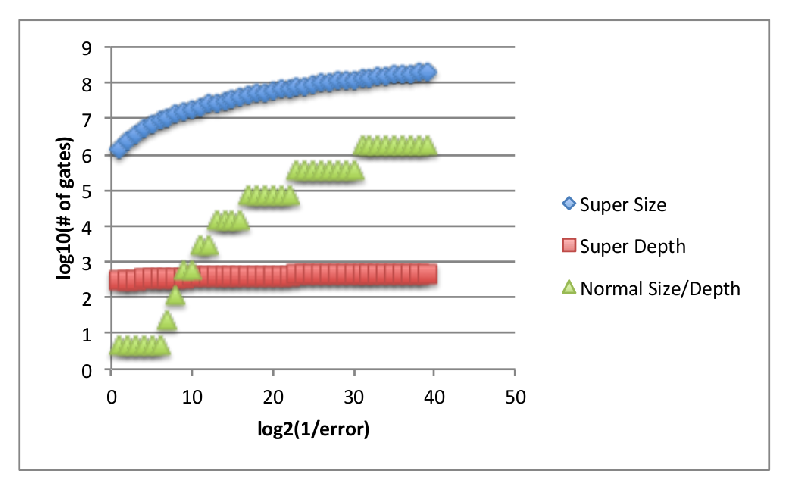
\includegraphics[width=3in]{circuit-size-depth.eps}
\caption{Compiled circuit size and depth}
\end{figure}
\end{center}

The tradeoff between Solovay-Kitaev and Super-Kitaev can most clearly
be seen in the use of space. Solovay-Kitaev uses no ancillae at run-time,
but requires a classical preprocessing step to generate basic
approximations (precompiled sequences from the universal set). Although
we did not generate sequences beyond $l_0 = 9$ for $SU(4)$, the curve
indicates it would soon require terabytes of storage, even if a more
efficient encoding were used (e.g. programming in C instead of Python).
Super-Kitaev, on the other hand, requires no preprocessing space, but
has a (currently intractable) requirement for ancilla qubits are run-time
which tracks the circuit size as $O(n^2 \log n)$.

\begin{center}
\begin{figure}[h!]
\label{fig:generation}
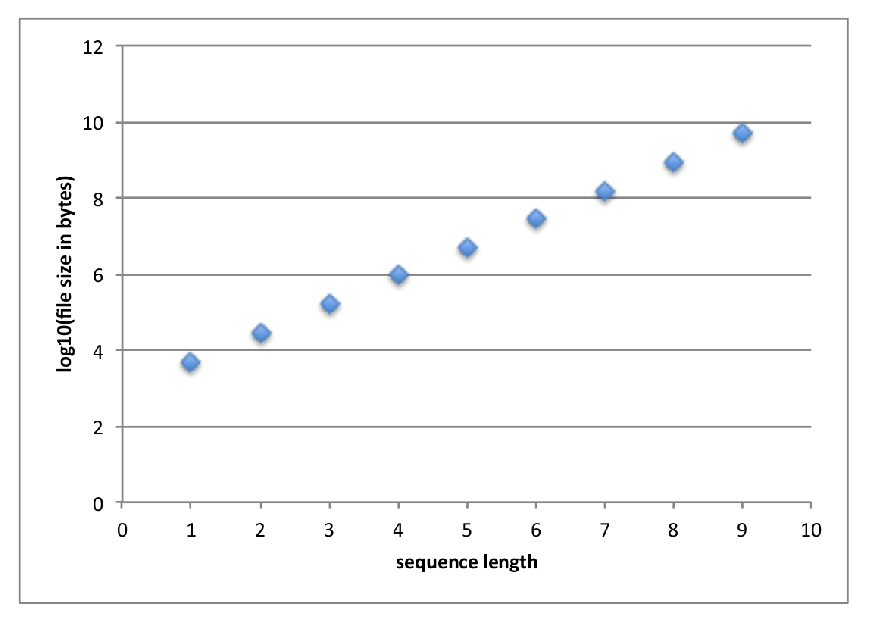
\includegraphics[width=3in]{normal-generation.eps}
\caption{Solovay-Kitaev preprocessing file sizes}
\end{figure}
\end{center}

\begin{center}
\begin{figure}[h!]
\label{fig:ancilla}
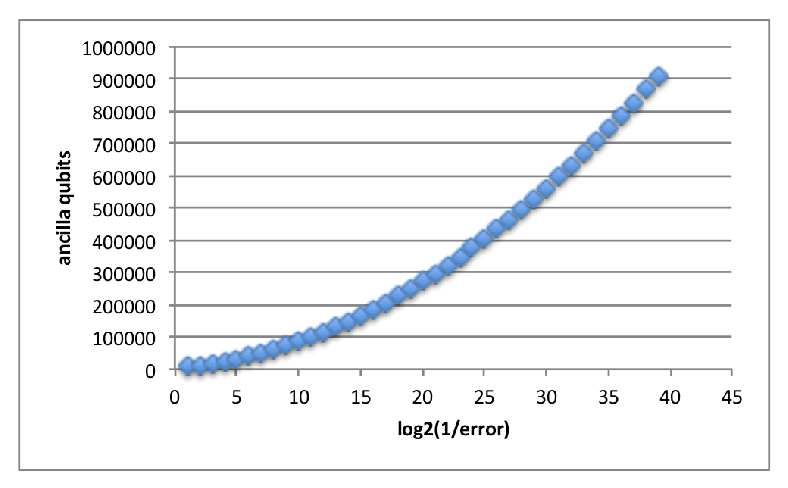
\includegraphics[width=3in]{super-ancilla.eps}
\caption{Super-Kitaev ancilla}
\end{figure}
\end{center}


\section{Conclusion and Future Directions}

In summary, we have seen the expected asymptotic bounds of both the
Solovay-Kitaev and Super-Kitaev quantum compiling algorithms reflected in
numerical resource comparisons. Solovay-Kitaev requires a large classical
preprocessing overhead but produces a more tractable number of compiled
gates and zero ancillae, albeit at larger circuit depth. This seems to be
a more reasonable choice for early experiments in running algorithms on an
80-qubit ion-trap quantum computer, where physical trapping constraints
make large numbers of qubits problematic but we are potentially willing to
wait a long time for the computation to complete. On the other hand, the
situation may change in the future when
quantum computers become more mature, scalable, and parallel;
when we become more ambitious in our
algorithm input sizes; and when the performance bottleneck becomes circuit depth.
In that case, Super-Kitaev may be preferrable.
Quantum computer engineers of the future will be able to use this work to
choose the most suitable quantum compiling technique currently available
as well as compare it to future compiling algorithms.

Moreover, the development of a compiler is intertwined with the
development of the underlying architecture. Just as classical programming
languages hint at what features would be desirable to move out of software
(and compile-time)
and into hardware (and run-time), Super-Kitaev provides some suggestions
to future quantum architectures. Hardware which seeks to take advantage of
this low-depth compiling would need to have a
"phase factory" for enacting the $\Lambda(e^{i\phi})$ gate, which would
included an efficient parallelized phase estimation routine. These are
novel resources which are currently not being considered in related literature.

Furthermore, quantum compiling may provide some hints to how we can program
their analog cousins. Although analog computers have fallen out of
favor as a primary computing model due to noise problems, they are making a
resurgence as a complementary ``coprocessor'' to digital computers, much like
the imagined future role of quantum computers. Like quantum computers,
analog computing uses existing physical properties to perform useful
computation, such as solving differential equations using electric current
and potential. Multiple AC signals and a single DC signal can coexist
in superposition on a wire,
and complex impedance from resistors, capacitors, and inductors
can differentiate between components of different frequencies.

\begin{displaymath}
V = I(R + \frac{1}{j\omega_1 C} + j\omega_2 L + \ldots)
\end{displaymath}

While it is unlikely that such a model would be more powerful in general
from a computational complexity point of view, we may be able to use them
as a practical aid in solving specific engineering problems, such as
encoding the periods of cyclic integer groups in corresponding periods of
sinusoidal signals. Such an analog computing model might be able to be
programmed via recursive successive approximation like Solovay-Kitaev or
using the techniques of Super-Kitaev.

\section{Acknowledgements}

The author would like to gratefully acknowledge the help of
his advisors Dave Bacon and Mark Oskin,
as well as Aram Harrow for the introduction to
Super-Kitaev and related expertise.

\bibliography{report}
\bibliographystyle{tocplain}

\end{document}
